%==================================================
% RESULTADOS DEL ANÁLISIS
%==================================================

\ReportChapter{Resultados del Análisis}

Los resultados presentados en esta sección muestran los principales hallazgos obtenidos durante el proceso de análisis. Cada apartado desarrolla un aspecto específico del comportamiento financiero estudiado mediante evidencia cuantitativa, visualizaciones e interpretación de resultados.



%==================================================
% ANÁLISIS 1
%==================================================

\SectionTitle{Caracterización general de la cartera crediticia}

El análisis inicial permite identificar la composición de la cartera y las principales características de los clientes evaluados, estableciendo una visión general del comportamiento financiero observado.



%--------------------------------------------------
% Tabla 1
%--------------------------------------------------

\textbf{\color{ReportGold}Tabla 1.} Caracterización general de la cartera crediticia


\vspace{0.3cm}

% Archivo generado automáticamente. No editar a mano.
\begin{table}[htbp]
\centering
\begin{adjustbox}{max width=\textwidth}
\begin{tabular}{lccc}
\toprule
 & fecha & saldo & fecha\_str \\
\midrule
0 & 2025-01-01 00:00:00 & 1659555.47 & 01-01-2025 \\
1 & 2025-02-01 00:00:00 & 2413002.99 & 01-02-2025 \\
2 & 2025-03-01 00:00:00 & 2326675.34 & 01-03-2025 \\
3 & 2025-04-01 00:00:00 & 1877667.33 & 01-04-2025 \\
4 & 2025-05-01 00:00:00 & 2027743.77 & 01-05-2025 \\
... & ... & ... & ... \\
7 & 2025-08-01 00:00:00 & 2127324.14 & 01-08-2025 \\
8 & 2025-09-01 00:00:00 & 1895080.98 & 01-09-2025 \\
9 & 2025-10-01 00:00:00 & 1839979.38 & 01-10-2025 \\
10 & 2025-11-01 00:00:00 & 2144329.81 & 01-11-2025 \\
11 & 2025-12-01 00:00:00 & 2551370.28 & 01-12-2025 \\
\bottomrule
\end{tabular}

\end{adjustbox}
\caption{Resultado de la variable: \texttt{table_ques1}}
\label{tab:table_ques1}
\smallskip\textit{Mostrando las primeras 5 y últimas 5 filas de un total de 12 registros $\times$ 3 variables.}}
\end{table}



\vspace{0.5cm}

La información resumida en la tabla permite establecer los patrones principales de la cartera analizada. A partir de estos resultados se identifican diferencias relevantes entre los grupos considerados.



%--------------------------------------------------
% Figura 1
%--------------------------------------------------

\textbf{\color{ReportGold}Figura 1.} Distribución general de los indicadores asociados a la cartera crediticia.


\vspace{0.3cm}

\begin{figure}[H]
\centering
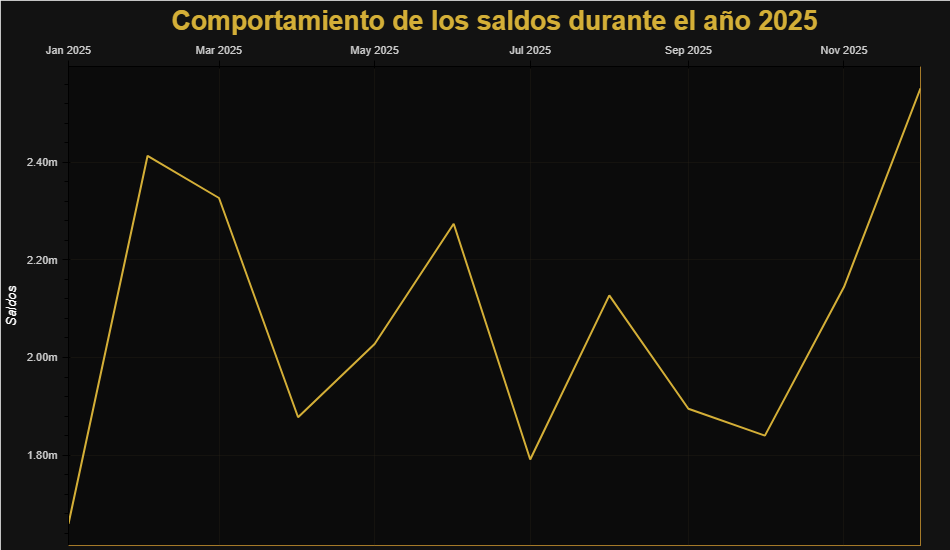
\includegraphics[width=0.90\textwidth]{../../../charts/chart_ques1.png}
\label{fig:cartera_general}
\end{figure}



\textbf{\color{ReportGold}Insight}

Análisis
La evolución mensual de los saldos bancarios durante 2025 evidencia un comportamiento caracterizado por fluctuaciones a lo largo del período analizado. El saldo total administrado por el banco oscila entre aproximadamente
Q1.79 millones
y
Q2.55 millones
, registrándose el valor más alto en el mes de diciembre, lo que representa una variación cercana a
Q800 mil
entre el valor mínimo y el máximo observado.
No se identifica una tendencia sostenida de crecimiento o disminución durante el año. En su lugar, los saldos presentan variaciones mensuales que podrían estar asociadas a factores estacionales o a cambios en el comportamiento financiero de los clientes.
El incremento registrado en diciembre podría estar relacionado con eventos propios de la época, como el pago de aguinaldos, bonos, remesas o un mayor dinamismo de la actividad económica. No obstante, confirmar estas hipótesis requeriría incorporar información adicional, como indicadores macroeconómicos o campañas comerciales desarrolladas por la institución durante el mismo período.



\clearpage



%==================================================
% ANÁLISIS 2
%==================================================

\SectionTitle{Factores asociados al riesgo crediticio}

El análisis de los factores relacionados con el riesgo permite evaluar qué características presentan mayor relación con el comportamiento observado en la cartera.



%--------------------------------------------------
% Tabla 2
%--------------------------------------------------

\textbf{\color{ReportGold}Tabla 2.} Factores asociados al riesgo crediticio


\vspace{0.3cm}

% Archivo generado automáticamente. No editar a mano.
\begin{table}[htbp]
\centering
\begin{adjustbox}{max width=\textwidth}
\begin{tabular}{lrr}
\toprule
 & agencia & saldo \\
\midrule
0 & Zona 10 & 4713085.480000 \\
1 & Cobán & 4803674.040000 \\
2 & Quetzaltenango & 4920131.860000 \\
3 & Escuintla & 5152377.070000 \\
4 & Petén & 5338387.170000 \\
\bottomrule
\end{tabular}
\end{adjustbox}
\caption{Análisis de datos: Table Ques2}
\label{tab:table_ques2}
\vspace{0.15cm}
\raggedright{\sffamily\footnotesize\color{CorporateGray}
\textit{Nota: Conjunto completo de datos (5 registros $\times$ 2 variables).}}
\end{table}



\vspace{0.5cm}

Los resultados obtenidos permiten identificar las variables con mayor relevancia dentro del análisis. La representación gráfica complementa la información cuantitativa y facilita la interpretación de los patrones encontrados.



%--------------------------------------------------
% Figura 2
%--------------------------------------------------

\textbf{\color{ReportGold}Figura 2.} Relación entre los principales factores asociados al riesgo crediticio.


\vspace{0.3cm}

\begin{figure}[H]
\centering
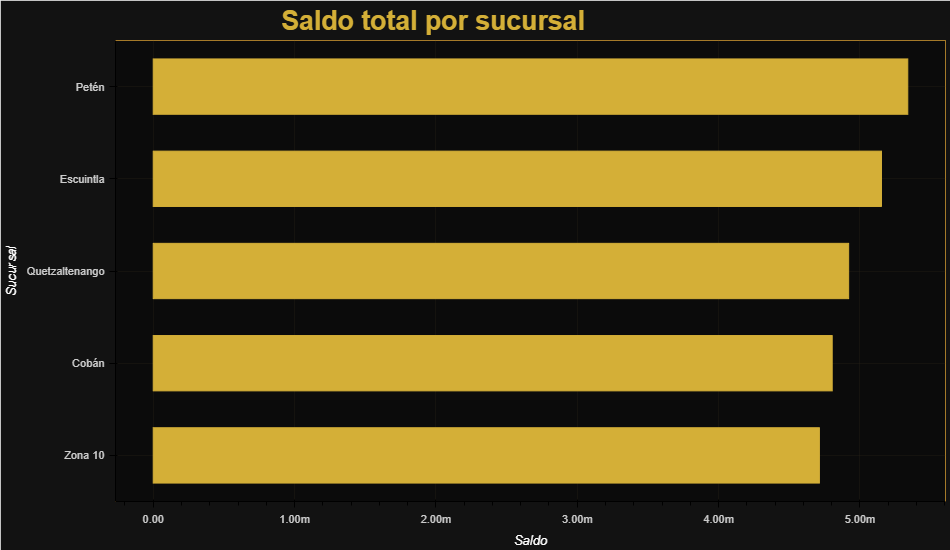
\includegraphics[width=0.90\textwidth]{../../../charts/chart_ques2.png}
\label{fig:factores_riesgo}
\end{figure}



\textbf{\color{ReportGold}Insight}

Análisis
La distribución del saldo total administrado por las agencias presenta diferencias moderadas entre las cinco sucursales analizadas. La agencia de
Petén
concentra el mayor volumen de saldos, con aproximadamente
Q5.34 millones
, mientras que la agencia ubicada en
Zona 10
registra el menor saldo agregado, con alrededor de
Q4.71 millones
. La diferencia entre ambas asciende a aproximadamente
Q500 mil
, lo que representa una variación relativamente reducida considerando el volumen total administrado por cada sucursal.
En términos generales, no se observa una concentración significativa de los saldos en una única agencia. Los resultados reflejan una distribución relativamente equilibrada entre las sucursales, lo que sugiere que la cartera de clientes y los recursos administrados no dependen de forma predominante de una sola ubicación geográfica.
Un aspecto que merece un análisis más detallado es que las agencias ubicadas fuera del área metropolitana presentan niveles de saldos comparables e incluso superiores a la sucursal de Zona 10. Este comportamiento podría estar asociado a diversos factores, como la composición de la cartera de clientes, la presencia de actividades económicas relevantes en dichas regiones, el nivel de bancarización o estrategias comerciales específicas implementadas por la institución. No obstante, la información disponible no permite establecer una relación causal, por lo que sería necesario incorporar variables adicionales para explicar este patrón con mayor precisión.



\clearpage



%==================================================
% ANÁLISIS 3
%==================================================

\SectionTitle{Comportamiento del crédito según características del cliente}

El análisis segmentado permite evaluar diferencias en el comportamiento crediticio según las características particulares de los clientes.



%--------------------------------------------------
% Tabla 3
%--------------------------------------------------

\textbf{\color{ReportGold}Tabla 3.} Comportamiento crediticio según características del cliente


\vspace{0.3cm}

% Archivo generado automáticamente. No editar a mano.
\begin{table}[htbp]
\centering
\begin{adjustbox}{max width=\textwidth}
\begin{tabular}{ll}
\toprule
segmento & saldo \\
\midrule
Adulto & 8012228.33 \\
Joven & 8339027.73 \\
Premium & 8576399.56 \\
\bottomrule
\end{tabular}
\end{adjustbox}
\caption{Table Ques3}
\label{tab:table_ques3}
\vspace{0.15cm}
\raggedright{\sffamily\footnotesize\color{ThemeMuted}
\textit{Nota: Conjunto completo de datos (3 registros $\times$ 2 variables).}}
\end{table}



\vspace{0.5cm}

La tabla presenta los principales indicadores utilizados para comparar los segmentos analizados, mientras que la visualización permite observar diferencias y tendencias relevantes.



%--------------------------------------------------
% Figura 3
%--------------------------------------------------

\textbf{\color{ReportGold}Figura 3.} Comportamiento crediticio según características del cliente.


\vspace{0.3cm}

\begin{figure}[H]
\centering
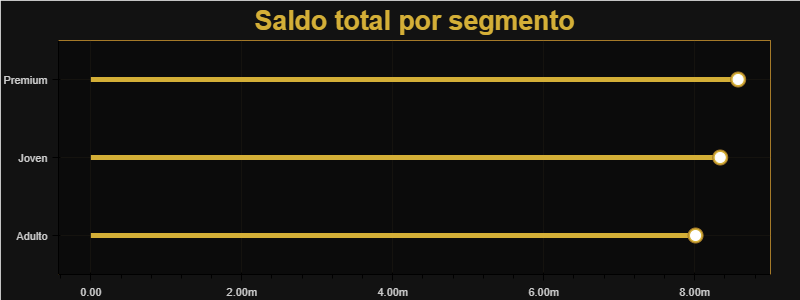
\includegraphics[width=0.90\textwidth]{../../../charts/chart_ques3.png}
\label{fig:segmentacion_cliente}
\end{figure}



\textbf{\color{ReportGold}Insight}

Análisis
La distribución del saldo por segmento de clientes muestra una composición relativamente equilibrada entre los tres grupos analizados. El segmento
Premium
concentra el mayor volumen de saldos, con aproximadamente
Q8.58 millones
, seguido por el segmento
Joven
con
Q8.34 millones
y, finalmente, el segmento
Adulto
, con alrededor de
Q8.01 millones
. La diferencia entre el segmento con mayor y menor saldo es cercana a
Q500 mil
, lo que evidencia una variación moderada entre ellos.
En términos generales, no se observa una concentración marcada de los saldos en un único segmento de clientes. Los resultados reflejan una distribución relativamente homogénea, lo que sugiere que el banco mantiene una cartera diversificada y que su volumen de recursos administrados no depende exclusivamente de un perfil específico de clientes.
Aunque el segmento
Premium
registra el mayor saldo agregado, la diferencia respecto a los demás segmentos es reducida. Este comportamiento podría indicar que las estrategias de captación y retención de clientes han logrado una distribución equilibrada de los recursos entre los distintos perfiles. Sin embargo, para comprender las causas de esta distribución sería necesario complementar el análisis con información adicional, como el número de clientes por segmento, el saldo promedio por cliente y la evolución temporal de cada grupo.



\clearpage



%==================================================
% ANÁLISIS 4
%==================================================

\SectionTitle{Evolución temporal del comportamiento financiero}

El análisis histórico permite identificar cambios en el comportamiento de la cartera y posibles periodos de variación significativa.



%--------------------------------------------------
% Tabla 4
%--------------------------------------------------

\textbf{\color{ReportGold}Tabla 4.} Evolución temporal del comportamiento financiero


\vspace{0.3cm}

% Archivo generado automáticamente. No editar a mano.
\begin{table}[htbp]
\centering
\begin{adjustbox}{max width=\textwidth}
\begin{tabular}{lcccc}
\toprule
 & cliente\_id & ingreso & saldo & segmento \\
\midrule
0 & 1 & 3819.00 & 24522.72 & Premium \\
1 & 2 & 20870.00 & 35735.08 & Joven \\
2 & 3 & 22726.00 & 32879.64 & Adulto \\
3 & 4 & 12115.00 & 25499.88 & Premium \\
4 & 5 & 8094.00 & 29405.95 & Joven \\
... & ... & ... & ... & ... \\
995 & 996 & 27776.00 & 24017.37 & Adulto \\
996 & 997 & 26273.00 & 751.93 & Joven \\
997 & 998 & 19075.00 & 46664.96 & Adulto \\
998 & 999 & 18186.00 & 28385.92 & Adulto \\
999 & 1000 & 18484.00 & 37629.65 & Adulto \\
\bottomrule
\end{tabular}

\end{adjustbox}
\caption{Resultado de la variable: \texttt{table_ques4}}
\label{tab:table_ques4}
\smallskip\textit{Mostrando las primeras 5 y últimas 5 filas de un total de 1,000 registros $\times$ 4 variables.}}
\end{table}



\vspace{0.5cm}

Los resultados permiten observar la evolución de los indicadores analizados y establecer patrones temporales relevantes.



%--------------------------------------------------
% Figura 4
%--------------------------------------------------

\textbf{\color{ReportGold}Figura 4.} Evolución temporal de los indicadores financieros analizados.


\vspace{0.3cm}

\begin{figure}[H]
\centering
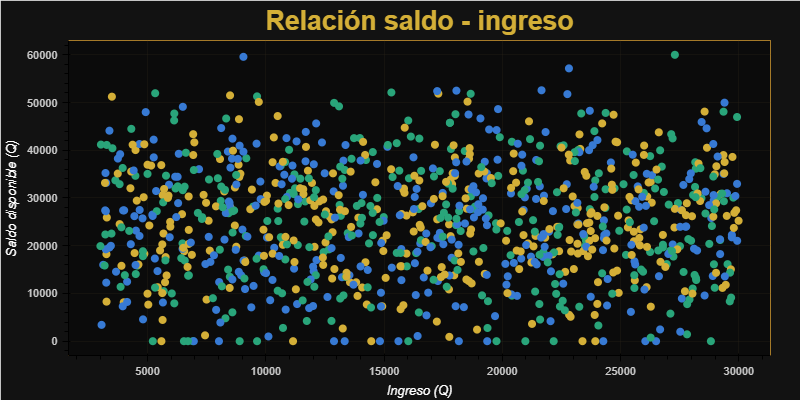
\includegraphics[width=0.90\textwidth]{../../../charts/chart_ques4.png}
\label{fig:evolucion_temporal}
\end{figure}



\textbf{\color{ReportGold}Insight}

Análisis
El análisis de la relación entre el ingreso de los clientes y el saldo disponible en sus cuentas no evidencia un patrón lineal claramente definido. La dispersión de las observaciones muestra que clientes con niveles de ingreso similares pueden presentar saldos considerablemente diferentes y, de igual forma, clientes con ingresos elevados no necesariamente mantienen los saldos más altos. Este comportamiento se observa tanto en el conjunto de datos como al diferenciar los registros por segmento de clientes.
La distribución de los datos sugiere que el nivel de ingreso, por sí solo, no constituye un factor suficiente para explicar el comportamiento de los saldos bancarios. La ausencia de una tendencia claramente definida indica que podrían intervenir otros elementos que no se encuentran representados en la base de datos, tales como los hábitos de ahorro, la antigüedad del cliente, el uso de productos financieros, la actividad económica o características particulares de cada cliente.
A partir de este resultado, sería recomendable complementar el análisis mediante técnicas estadísticas, como el cálculo del coeficiente de correlación o la estimación de un modelo de regresión, con el fin de cuantificar la intensidad de la relación entre ambas variables y evaluar si esta resulta estadísticamente significativa. Asimismo, la incorporación de variables adicionales permitiría desarrollar un análisis multivariado que explique con mayor precisión los factores asociados al comportamiento de los saldos bancarios.



\clearpage



%==================================================
% ANÁLISIS 5
%==================================================

\SectionTitle{Identificación de patrones relevantes del riesgo}

El análisis final integra los resultados obtenidos para identificar patrones generales asociados al comportamiento crediticio.



%--------------------------------------------------
% Tabla 5
%--------------------------------------------------

\textbf{\color{ReportGold}Tabla 5.} Identificación de patrones relevantes del riesgo


\vspace{0.3cm}


% Archivo generado automáticamente. No editar manualmente.

\begin{table}[htbp]

\centering

\begin{adjustbox}{max width=\textwidth}

\begin{tabular}{ll}

\rowcolor{ThemeBackground}
\rule{0pt}{0.45cm}
\textcolor{ThemeGold}{\bfseries grupo\_edad} & \textcolor{ThemeGold}{\bfseries saldo} \\

15-19 & 790852.56 \\
20-24 & 2666010.58 \\
25-29 & 2407436.99 \\
30-34 & 2179591.76 \\
35-39 & 2146435.52 \\
... & ... \\
50-54 & 2626315.58 \\
55-59 & 2144247.86 \\
60-64 & 2701876.70 \\
65-69 & 2327534.66 \\
70-74 & 464016.31 \\
\bottomrule
\end{tabular}

\end{adjustbox}

\vspace{0.15cm}
{\raggedright\sffamily\footnotesize\color{ThemeMuted}
\textit{Nota: Se muestran las primeras y últimas 5 filas. Conjunto completo: 12 registros $\times$ 2 variables.}}

\end{table}



\vspace{0.5cm}

La evidencia presentada permite sintetizar los principales hallazgos encontrados durante el estudio y establecer relaciones entre las variables evaluadas.



%--------------------------------------------------
% Figura 5
%--------------------------------------------------

\textbf{\color{ReportGold}Figura 5.} Patrones generales identificados en el análisis del riesgo crediticio.


\vspace{0.3cm}

\begin{figure}[H]
\centering
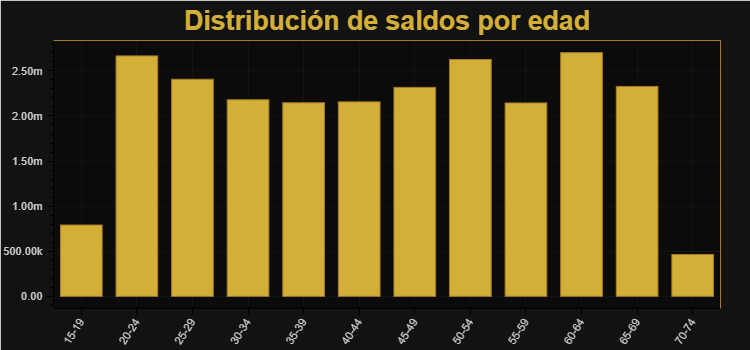
\includegraphics[width=0.90\textwidth]{../../../charts/chart_ques5.png}
\label{fig:patrones_riesgo}
\end{figure}



\textbf{\color{ReportGold}Insight}

Análisis
La distribución de los saldos por rango de edad durante 2025 muestra que la mayor concentración de recursos se encuentra en los clientes con edades comprendidas entre
20 y 69 años
. En estos grupos, el saldo agregado oscila entre aproximadamente
Q2.15 millones
y
Q2.70 millones
, evidenciando una distribución relativamente homogénea entre las diferentes etapas de la vida laboral.
Por el contrario, los grupos ubicados en los extremos de la distribución, correspondientes a clientes de
15 a 19 años
y de
70 a 74 años
, registran los menores niveles de saldo, con montos aproximados entre
Q464 mil
y
Q790 mil
. La diferencia respecto a los grupos de mayor concentración resulta considerable, lo que sugiere una menor participación de estos rangos de edad en el volumen total de recursos administrados por el banco.
Este comportamiento es consistente con el ciclo de vida financiero de los clientes, ya que las edades comprendidas entre los 20 y 69 años suelen concentrar una mayor participación en el mercado laboral y, por consiguiente, una mayor capacidad para generar y mantener saldos en sus cuentas. No obstante, esta interpretación constituye una hipótesis de negocio y requeriría información adicional, como el número de clientes por rango de edad, el saldo promedio por cliente y otras variables socioeconómicas, para ser validada.